\section*{Exercises for Section~\ref{S:directproof}}

\begin{enumerate}
  \xitem Prove each of the following statements:  \label{exer:sec31-prove}
\begin{enumerate}
  \item For all integers  $a$, $b$, and  $c$   with $a \ne 0$,  if  $a \mid b$ and $a \mid c$, then $a \mid \left(b-c \right) $.\label{exer:sec31-provea}
  \item For each $n \in \Z$, if  $n$ is an odd integer, then $ n^3 $ is an odd integer.
  \item For each integer $a$, if 4 divides $(a - 1)$, then 4 divides $\left( a^2 - 1 \right)$.
\end{enumerate}


\item For each of the following, use a counterexample to prove the statement is false.
\begin{enumerate}
  \yitem For each odd natural number $n$, if $n > 3$, then 3 divides $\left( n^2 - 1 \right)$.
  \item For each natural number $n$, $\left( 3 \cdot 2^n + 2 \cdot 3^n + 1 \right)$ is a prime number.
  \item For all real numbers $x$ and $y$, $\sqrt{x^2 + y^2} > 2xy$.
  \yitem For each integer $a$, if 4 divides $\left( a^2 - 1 \right)$, then 4 divides $(a - 1)$.
\end{enumerate}


\item Determine if each of the following statements is true or false.  If a statement is true, then write a formal proof of that statement, and if it is false, then provide a counterexample that shows it is false.
\label{exer:3truefalse}%

\begin{enumerate}
\item For all integers $a$, $b$, and $c$ with $a \ne 0$, if $ a \mid b $, then 
$ a \mid \left(bc \right) $.
\label{exer:divprod}%

\yitem For all integers $a$ and  $b$ with $a \ne 0$,  if $ 6 \mid \left(ab \right) $, then 
$ 6 \mid a$ or $ 6 \mid b$.

\item For all integers $a$, $b$, and $c$ with $a \ne 0$, if $a$ divides $(b - 1)$ and $a$ divides 
$(c - 1)$, then $a$ divides $(bc - 1)$.

\yitem For each integer $n$, if 7 divides $\left( n^2 - 4 \right)$, then 7 divides $(n - 2)$.

\yitem For every integer $n$, $4n^2 + 7n + 6$ is an odd integer.

\yitem For every odd integer $n$, $4n^2 + 7n + 6$ is an odd integer.

\yitem For all integers $a$, $b$, and  $d$  with $d \ne 0$,  if  $d$   divides both  $a-b$  and  
$a+b$, then  $d$  divides  $a$.

\item For all integers $a$, $b$, and $c$ with $a \ne 0$, if $a \mid (bc)$, then $a \mid b$ or 
$a \mid c$.
\end{enumerate}


\xitem \begin{enumerate} \item If $x$ and $y$ are integers and $ xy=1$, explain why $ x=1$ or 
$ x=-1$.
  \item Is the following proposition true or false?

  \begin{list}{}
    \item For all nonzero integers $a$ and $b$, if $ a \mid b$ and $ b \mid a $, then 
$ a = \pm b $.\label{exer:diveachb}
  \end{list}
  \end{enumerate}
  \label{exer:diveach}%




\xitem Prove the following proposition:
\label{exer:sec31-10}%

  \begin{list}{}
    \item Let  $a$  be an integer.  If there exists an integer  $n$  such that \linebreak 
$ a \mid \left(4n+3 \right)$ and $ a \mid \left( 2n+1 \right) $, then  $a = 1$ or  
$a =  - 1$.
  \end{list}
\hint  Use the fact that the only divisors of 1 are 1 and $-1$.


\item Determine if each of the following statements is true or false.  If a statement is true, then write a formal proof of that statement, and if it is false, then provide a counterexample that shows it is false.
\begin{enumerate}
    \item For each integer $a$, if there exists an integer $n$ such that $a$ divides $(8n + 7)$ and $a$ divides 
$(4n + 1)$, then $a$ divides 5.
  \item For each integer $a$, if there exists an integer $n$ such that $a$ divides $(9n + 5)$ and $a$ divides 
$(6n + 1)$, then $a$ divides 7.
  \item For each integer $n$, if $n$ is odd, then 8 divides $\left( n^4 + 4n^2 + 11 \right)$.
  \item For each integer $n$, if $n$ is odd, then 8 divides $\left( n^4 + n^2 + 2n \right)$.
\end{enumerate}



\item Let  $a$ be an integer and let $n \in \mathbb{N}$.  

  \begin{enumerate}
    \item Prove that if  $a \equiv 0 \pmod n$, then $ n \mid a $.
    \item Prove that if  $ n \mid a $, then  $a \equiv 0 \pmod n$.
  \end{enumerate}


\xitem Let $a$ and $b$ be integers.  Prove that if $a \equiv 2 \pmod 3$ and $b \equiv 2 \pmod 3$, then
\label{exer:congmod3}%

\begin{multicols}{2}
\begin{enumerate}
\item $a + b \equiv 1 \pmod 3$;

\item $a \cdot b \equiv 1 \pmod 3$.
\end{enumerate}
\end{multicols}

\item Let $a$ and $b$ be integers.  Prove that if $a \equiv 7 \pmod 8$ and $b \equiv 3 \pmod 8$, then:

\begin{multicols}{2}
\begin{enumerate}
\item $a + b \equiv 2 \pmod 8$;

\item $a \cdot b \equiv 5 \pmod 8$.
\end{enumerate}
\end{multicols}

\item Determine if each of the following propositions is true or false.  Justify each conclusion.

\begin{enumerate}
\item For all integers $a$ and $b$, if $ab \equiv 0 \pmod 6$, then $a \equiv 0 \pmod 6$ or  
$b \equiv 0 \pmod 6$. 
\item For each integer $a$, if $a \equiv 2 \pmod 8$, then $a^2 \equiv 4 \pmod 8$.
\item For each integer $a$, if $a^2 \equiv 4 \pmod 8$, then $a \equiv 2 \pmod 8$.
\end{enumerate}

\newpage
%\xitem Prove the symmetric property of congruence stated in Theorem~\ref{T:modprops}.
%\label{exer:cong-symm}%
\item Let  $n$ be a natural number.  Prove each of the following:   \label{exer:cong-props}
\begin{enumerate}
  \yitem For every integer  $a$,  $a \equiv a \pmod n$. \label{exer:cong-reflexive}

This is called the \textbf{reflexive property}
\index{congruence!reflexive property}%
 of congruence modulo $n$.

  \yitem For all integers $a$ and $b$, if  $a \equiv b \pmod n$, then  $b \equiv a \pmod n$.

This is called the \textbf{symmetric property} \label{exer:cong-symmetry}
\index{congruence!symmetric property}%
 of congruence modulo $n$.

  \item For all integers $a$, $b$, and $c$, if  $a \equiv b \pmod n$ and $b \equiv c \pmod n$, then  
$a \equiv c \pmod n$.

This is called the \textbf{transitive property}
\index{congruence!transitive property}%
 of congruence modulo $n$.
\end{enumerate}


\xitem Let  $n$  be a natural number and let  $a$, $b$, $c$, and  $d$  be integers.  Prove each of the following.
\label{exer:sec31-11}%

  \begin{enumerate}
    \item If  $a \equiv b \pmod n$ and  $c \equiv d \pmod n$, then  \\$\left( {a + c} \right) \equiv \left( {b + d} \right) \pmod n$.
    \item If  $a \equiv b \pmod n$ and  $c \equiv d \pmod n$, then  
$ac \equiv bd \pmod n$.
\label{exer:congprops}%
  \end{enumerate}


\item  \label{exer:quadformula2} 
\begin{enumerate}
\item Let $a$, $b$, and $c$ be real numbers with $a \ne 0$.  Explain how to use a part of the quadratic formula (called the discriminant) to determine if the quadratic equation 
\index{quadratic equation}% 
 $ax^2 + bx + c = 0$ has two real number solutions, one real number solution, or no real number solutions.  (See Exercise~(\ref{exer:sec12-11}) in Section~\ref{S:direct} for a statement of the quadratic formula.)

\item Prove that if $a$, $b$, and $c$ are real numbers for which $a>0$ and \mbox{$c<0$}, then one solution of the quadratic equation
\mbox{$ax^2+bx+c=0$}
is a positive real number.

\item Prove that if  $a$, $b$, and  $c$  are real numbers, if  $a \ne 0$, $b > 0$ and %\linebreak
\mbox{$\dfrac{b}{2} < \sqrt {ac} $}, then the quadratic equation  $ax^2  + bx + c = 0$ has no real number solution.
\end{enumerate}


\item Let $h$ and $k$ be real numbers and let $r$ be a positive number.  The equation for a circle whose center is at the point $\left( h, k \right)$ and whose radius is $r$ is
\label{exer:circle-31}%

\[
\left( x - h \right)^2 + \left( y - k \right)^2 = r^2.
\]

\noindent
We also know that if $a$ and $b$ are real numbers, then

\begin{itemize}
\item The point $\left( a, b \right)$ is inside the circle if 
$\left( a - h \right)^2 + \left( b - k \right)^2 < r^2$.
\item The point $\left( a, b \right)$ is on the circle if 
$\left( a - h \right)^2 + \left( b - k \right)^2 = r^2$.
\item The point $\left( a, b \right)$ is outside the circle if 
$\left( a - h \right)^2 + \left( b - k \right)^2 > r^2$.
\end{itemize}

\noindent
Prove that all points on or inside the circle whose equation is 
$\left( x - 1 \right)^2 + \left( y - 2 \right)^2 = 4$ are inside the circle whose equation is 
$x^2 + y^2 = 26$.


\item \label{exer:insidecircle} Let $r$ be a positive real number. The equation for a circle of radius $r$ whose center is the origin is $x^2 + y^2 = r^2$.

\begin{enumerate}
\item Use implicit differentiation to determine $\dfrac{dy}{dx}$.

\item Let $\left(a, b \right)$ be a point on the circle with $a \ne 0$ and $b \ne 0$.  Determine the slope of the line tangent to the circle at the point $\left(a, b \right)$.

\item Prove that the radius of the circle to the point $\left(a, b \right)$ is perpendicular to the line tangent to the circle at the point $\left(a, b \right)$. \hint Two lines (neither of which is horizontal) are perpendicular if and only if the products of their slopes is equal to $-1$.
\end{enumerate}

\item Determine if each of the following statements is true or false.  Provide a counterexample for statements that are false and provide a complete proof for those that are true. 
\label{exer:AGM}%
\begin{enumerate}
\item For all real numbers $x$ and $y$, $\sqrt{xy} \leq \dfrac{x + y}{2}$.
\item For all real numbers $x$ and $y$, $xy \leq \left( \dfrac{x + y}{2} \right)^2$.
\item For all nonnegative real numbers $x$ and $y$, $\sqrt{xy} \leq \dfrac{x + y}{2}$.
\end{enumerate}

\item Use one of the true inequalities in Exercise~(\ref{exer:AGM}) to prove the following proposition.

\begin{list}{}
\item For each real number $a$, the value of $x$ that gives the maximum value of 
$y = x \left( a - x \right)$ is $x = \dfrac{a}{2}$.
\end{list}


\item \begin{enumerate}\label{exer:sec31-pythag}
\item State the Pythagorean Theorem for right triangles.

The diagrams in Figure~\ref{fig:for-exer-pythag} will be used for the problems in this exercise.
\begin{figure}[h]
\begin{center}
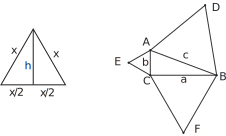
\includegraphics{figps-pythag-triangle}
\end{center}
\caption{Diagrams for Exercise~(\ref{exer:sec31-pythag})}
\label{fig:for-exer-pythag}
\end{figure} 

\item In the diagram on the left,  $x$  is the length of a side of the equilateral triangle and  
$h$  is the length of an altitude of the equilateral triangle.  The labeling in the diagram shows the fact that the altitude intersects the base of the equilateral triangle at the midpoint of the base.
Use the Pythagorean Theorem to prove that the area of this equilateral triangle is 
$\dfrac{\sqrt{3}}{4}x^2$.
%\begin{figure}[h]
%\begin{center}
%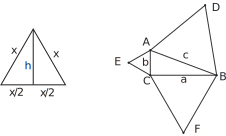
\includegraphics{figps-pythag-triangle}
%\end{center}
%\end{figure} 
\item In the diagram on the right, $\triangle ABC$ is a right triangle.  In addition, there has been an equilateral triangle constructed on each side of this right triangle.  Prove that the area of the equilateral triangle on the hypotenuse is equal to the sum of the areas of the equilateral triangles constructed on the other two sides of the right triangle.
%\begin{figure}[h]
%\begin{center}
%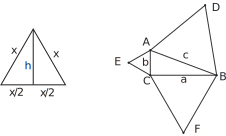
\includegraphics{figps-pythag-triangle}
%\end{center}
%\end{figure} 
\end{enumerate}




  \item \textbf{Evaluation of proofs} \hfill \\
This type of exercise will appear frequently in the book.  In each case, there is a proposed proof of a proposition.  However, the proposition may be true or may be false. 
\label{exer:proofeval}%

\begin{itemize}
\item If a proposition is false, the proposed proof is, of course, incorrect.  In this situation, you are to find the error in the proof and then provide a counterexample showing that the proposition is false.

\item If a proposition is true, the proposed proof may still be incorrect.  In this case, you are to determine why the proof is incorrect and then write a correct proof using the writing guidelines that have been presented in this book.

\item If a proposition is true and the proof is correct, you are to decide if the proof is well written or not.  If it is well written, then you simply must indicate that this is an excellent proof and needs no revision.  On the other hand, if the proof is not well written, then you must then revise the proof by writing it according to the guidelines presented in this text.
\end{itemize}

\begin{enumerate}
\item \textbf{Proposition}. If $m$ is an even integer, then $\left(5m + 4\right)$ is an even integer.

\begin{myproof}
We see that $5m + 4 = 10n + 4 = 2 \left(5n + 2 \right)$.  Therefore, $\left(5m + 4 \right)$ is an even integer.
\end{myproof}


\item \textbf{Proposition}. For all real numbers $x$ and $y$, if $x \ne y$, $x > 0$, and $y >0$, then $\dfrac{x}{y} + \dfrac{y}{x} > 2$.

\begin{myproof}
Since $x$ and $y$ are positive real numbers, $xy$ is positive and we can multiply both sides of the inequality by $xy$ to obtain
\begin{align*}
\left( \frac{x}{y} + \frac{y}{x} \right) \cdot xy &> 2 \cdot xy \\
                                        x^2 + y^2 &> 2xy.
\end{align*}
By combining all terms on the left side of the inequality, we see that 
$x^2 - 2xy + y^2 > 0$ and then by factoring the left side, we obtain 
$\left( x - y \right)^2 > 0$.  Since $x \ne y$, $\left(x - y \right) \ne 0$ and so 
$\left( x - y \right)^2 > 0$.  This proves that if $x \ne y$, $x > 0$, and $y >0$, then 
$\dfrac{x}{y} + \dfrac{y}{x} > 2$.
\end{myproof}

%\item \textbf{Proposition}. For all real numbers $x$ and $y$,  
%$xy \leq \left( \dfrac{x + y}{2} \right)^2$.
%
%\begin{myproof}
%If we expand the right side of the inequality, we obtain
%\[
%xy \leq \frac{x^2 + 2xy + y^2}{4}.
%\]
%Multiplying both sides of this inequality by 4 and then combining terms on the right sides of the inequality, we see that
%\begin{align*}
%4xy &\leq x^2 + 2xy + y^2 \\
%  0 &\leq x^2 - 2xy + y^2
%\end{align*}
%The right sides of the last inequality is a perfect square, and we see that 
%$0 \leq \left(x - y \right)^2$.  This proves that if $x$ and $y$ are real numbers, then 
%$xy \leq \left( \dfrac{x + y}{2} \right)^2$.
%\end{myproof}

%\item \textbf{Proposition}. If $m$ is an odd integer, then $\left(5m + 4\right)$ is an odd integer.
%
%\begin{myproof}
%Assume that $m$ is an odd integer.  Then, exists an integer $n$ such that
%\[
%m = 2n + 1.
%\]
%By multiplying both sides of this equation by 5, we see that $5m = 10n + 5$.  Hence,
%\[
%\begin{aligned}
%5m +4 &= 10n + 5 + 4 \\
%      &= 10n + 8 + 1 \\
%      &= 2 \left(5n + 4  \right) + 1.
%\end{aligned}
%\]
%By the closure properties of the integers, $\left(5n + 4 \right)$ is an integer, and hence, the last equation implies that $5m + 4$ is an odd integer.  This proves that if $m$ is an odd integer, then $5m + 4$ is an odd integer.
%\end{myproof}

\item \textbf{Proposition}. For all integers $a$, $b$, and $c$, if 
$a \mid \left( bc \right)$, then $a \mid b$ or $a \mid c$.

\begin{myproof}
We assume that $a$, $b$, and $c$ are integers and that $a$ divides $bc$.  So, there exists an integer $k$ such that $bc = ka$.
%\[
%bc = ka.
%\]
\noindent
We now factor $k$ as $k = mn$, where $m$ and $n$ are integers.  We then see that
\[
bc = mna.
\]
\noindent
This means that $b = ma$ or $c = na$ and hence, $a \mid b$ or $a \mid c$.
\end{myproof}

\item \textbf{Proposition}.  For all positive integers $a$, $b$, and $c$, 
$\left( a^b \right)^c = a^{\left( b^c \right)}$.

This proposition is false as is shown by the following counterexample:  If we let $a = 2$, $b = 3$, and $c = 2$, then
\begin{align*}
\left( a^b \right)^c &= a^{\left( b^c \right)} \\
\left( 2^3 \right)^2 &= 2^{\left( 3^2 \right)} \\
8^2 &= 2^9 \\
64 &\ne 512
\end{align*}
\end{enumerate}
\end{enumerate}

\subsection*{Explorations and Activities}
\setcounter{oldenumi}{\theenumi}
\begin{enumerate} \setcounter{enumi}{\theoldenumi}
%   \item \textbf{Exploring Some Congruences}.  Determine if each of the following statements is true or false.  This means that if a statement is true, then write a formal proof of that statement, and if it is false, then provide a counterexample that shows it is false.
%\begin{enumerate}   
%  \item For each integer $a$, $a \equiv 3 \pmod 7$ if and only if 
%$\left(a^2 + 5a \right) \equiv 3 \pmod 7$.
%
%  \item For each integer $a$, $a \equiv 2 \pmod 8$ if and only if 
%$\left(a^2 + 4a \right) \equiv 4 \pmod 8$.
%\end{enumerate}





  \item \textbf{Congruence Modulo 6}.  \begin{enumerate}
  \item Find several integers that are congruent to 5 modulo 6 and then square each of these integers.
\label{A:mod6-1}%

  \item For each integer  $m$  from Part~(\ref{A:mod6-1}), determine an integer  $k$  so that  $0 \leq k < 6$  and  $m^2  \equiv k \pmod 6$.  What do you observe?
\label{A:mod6-2}%

  \item Based on the work in Part~(\ref{A:mod6-2}), complete the following conjecture: 
\label{A:mod6-3}%

\begin{center}
For each integer $m$, if $m \equiv 5 \pmod 6$, then \ldots .
\end{center}

\item Complete a know-show table for the conjecture in Part~(\ref{A:mod6-3}) or write a proof of the conjecture. 
\end{enumerate}

\item \textbf{Pythagorean Triples}.  Three natural numbers $a$, $b$, and $c$ with $a < b < c$ are called a Pythagorean triple
\index{Pythagorean triple}%
 provided that $a^2 + b^2 = c^2$.  See Exercise~(\ref{exer31:pythagorean}) on page~\pageref{exer31:pythagorean} in Section~\ref{S:direct}.  Three natural numbers are called \textbf{consecutive natural numbers} if they can be written in the form $m$, $m + 1$, and $m + 2$, where $m$ is a natural number.

\vskip6pt
\noindent
\begin{enumerate}
  \item Determine all Pythagorean triples consisting of three consecutive natural numbers.  (State a theorem and prove it.)
  \item Determine all Pythagorean triples that can be written in the form $m$, $m + 7$, and $m + 8$, where $m$ is a natural number.  State a theorem and prove it.
%  \item Determine all Pythagorean triples that can be written in the form $m$, $m + 9$, and $m + 10$, where $m$ is a natural number.  State a theorem and prove it.
\end{enumerate}
\end{enumerate}

\hbreak
\endinput

